\chapter{Introduction}\label{sec:intro}
\begin{flushright}{\slshape
I choose a lazy person to do a hard job,\\
because a lazy person will find an easy way to do it.}\\
\medskip
--- Bill Gates
\end{flushright}

\noindent Since the dawn of time, humanity has always tried to find ways to make work easier. With the start of the industrial revolution, this was achieved by constructing machines and other helpful contraptions which automated a task. In more recent years, a guiding procedure - a process - was installed to streamline the workflow where complete automation was not possible. With the rise of the credo "what gets measured, gets managed", key performance indicators (KPIs) were installed into manual labor processes~\cite{web:taylorism-and-drucker} to optimize process efficiency further.\\

However, processes and KPIs fell short of penetrating and improving the realm of knowledge work, since the foundational mechanics of it differ strongly from manual labor. Peter F. Drucker, a renowned management educator, realized this in 1999:
"The most important contribution of management in the 20th century was to increase manual worker productivity fifty-fold. The most important contribution of management in the 21st century will be to increase knowledge worker productivity — hopefully by the same percentage"~\cite{drucker1999}.\\

In the spirit of Drucker's statement and by leveraging the technical developments of the years since his statement, we apply deep learning on business process data to predict the next activity in a running business process by using its execution history. We focus on deep learning methods because they have been shown to outperform others~\cite{tax2018interdisciplinary}. How this is a step toward process automation in knowledge work, will be explained further in \autoref{sec:intro:motivation}.  We highlight the resulting contribution to current research in \autoref{sec:intro:contribution}. The chapter ends in \autoref{sec:intro:outline} with a description of the thesis outline.

\section{Motivation} \label{sec:intro:motivation}
Automation of work is a phenomenon that has occurred in the past with manual labor and is spreading into other types of work today, namely knowledge work. As mentioned before, manual labor and knowledge work differ:

The course of manual labour is determined by physical laws, is often very structured, and thus offers great potential for simple automation - like work at an assembly line. Knowledge work, on the other hand, requires workers to "think for a living", and is strongly shaped by the individuality of the thoughts and habits of each knowledge worker~\cite{drucker1999}. As each worker has a different knowledge background and uses information differently, this type of work is very flexible and often no process is executed exactly the same~\cite{hewelt2016}. Popular examples of knowledge work are insurance claims, handled by several employees. Each claim requires a different course of action since the information contained in each case differs.\\

In the 20 years since Drucker's mission statement, the analog tools of knowledge workers have evolved into a plethora of digital systems and applications. These help make their decisions more informed and faster. Furthermore, these systems also track work progress, resulting in a large number of logs which document the course that work on a case, i.e. a running process, has taken.\\

These logs are a valuable source of information as they can reveal best practices that knowledge workers use in certain situations. If this data were processed, such best practices could be recommended by an auxiliary system. These knowledge worker assistance systems have been called for in recent literature reviews by Hauder et al.~\cite{hauder2014} and Francescomarino et al.~\cite{francescomarino2018}, but have only been implemented prototypically until now. One of the challenges that lie in the way of creating assistance systems is the task of anticipating the development of a case and foreseeing which part comes next. Once then a machine understands the \textit{what} and is only missing the \textit{how}, the ability to forecast process developments can be understood as a step toward process automation.\\

Forecasting the course of a running process can be useful for workers doing either manual labor or knowledge work. Manual labor is often dominated by questions of time and outcome~\cite{rogge2013} because the course of work is clear - natural interests in a world of distributed supply chains and just-in-time production~\cite{web:economist:jit}. The course of the work itself is of interest in the case of unstructured knowledge work~\cite{francescomarino2015}, which is often unclear and depends on the information handled inside a case. Knowing about the development of a case presents workers with an opportunity to intervene if it were to progress in an unwanted fashion.\\

By regarding the execution history of an ongoing case, the prediction of its next activity is possible - illustrated in \autoref{fig:next-activity-prediction}. This prediction could then be processed further by the aforementioned assistance system, e.g. to propose an intervention if a case takes an unwanted course. The application of Predictive Analytics on business processes enables this type of prediction. It is fairly new and is commonly referred to as Predictive Process Monitoring.

\begin{figure}
    \centering
    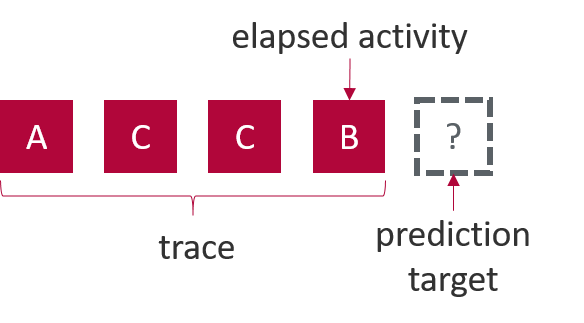
\includegraphics[width=0.7\textwidth]{gfx/next-activity.png}
    \caption[Next-activity prediction from a trace]{The next activity of a case is predicted from the sequence of elapsed activities in its trace}
    \label{fig:next-activity-prediction}
\end{figure}

We realized that the current research in this young domain can be improved in three areas. These will henceforth be referred to as improvement areas:

\begin{enumerate}
    \item[\textbf{Area 1}] Comparability: Published approaches often use different datasets, making them hard to compare.
    \item[\textbf{Area 2}] Reproducibility: Divergent approaches to training the prediction models and low technical depth of the publications make it hard to reproduce the published results. Furthermore, some prediction approaches are not focused on a single case but whole event streams without specific regard to a case~\cite{evermann2016, schoenig2018}.
    \item[\textbf{Area 3}] NLP-Influence: The history of a case is essentially a sequence, but little inspiration has been taken from Natural Language Processing (NLP), where sequence prediction is common~\cite{shibata2016bipartite}.
\end{enumerate}

\section{Contribution}\label{sec:intro:contribution}
In this work, we make a contribution to ongoing research by applying neural networks to process execution logs to predict the next activity. The work was guided by the three improvement areas.

We address Area 3 by reusing a successful sequence prediction approach from the NLP domain and applying it on business process log data. We also adapt it to incorporate learnings from a paper~\cite{klinkmuller2018reliablemonitoring}. We compare two models to reimplemented prediction models of two published approaches. This provides us with the direct comparability mentioned in Area 1. The models were reverse-engineered from the following publications:

\begin{enumerate}
    \item\textit{A Deep Learning Approach for Predicting Process Behaviour at Runtime} by Evermann et al.~\cite{evermann2016}
    \item\textit{Deep Learning Process Prediction with Discrete and Continuous Data Features} by Schönig et al.~\cite{schoenig2018}.
\end{enumerate}

Over the course of reverse-engineering the comparison models and the subsequent evaluation, widely divergent understandings and approaches with regard to the batch structure of sequential training data input for neural networks were uncovered. To contribute to a better understanding in this area, a comparison of four different batching strategies was incorporated into the evaluation.

As we remarked the comparability of current publications in Area 1, we include a sequence prediction model training framework in this thesis. It allowed us to train four different models with four different batching strategies on seven prepared datasets with ease. It is extensible for other researchers to facilitate comparability among future works.

We use the datasets from the Business Process Intelligence Competition (BPIC) years 2011, 2012, and 2015, where the latter consists of five datasets. The processes in each dataset differ strongly from each other, and we infer a suggestion on which batching strategy could be advantageous to use on which flavor of process log. The use of the BPIC12 dataset furthermore allows for a direct comparison to published next-activity prediction approaches.

We evaluate the trained models using three criteria: First, total accuracy. Second, we test for accuracy stability across the whole execution of the process, which we believe is key for putting trust into the model~\cite{francescomarino2015, boehmer2018probability}. Third, we investigate training time requirements.

From the three evaluation criteria, we reason about the effectiveness of certain model-batching-strategy combinations and finally compare them to published performance figures.

\section{Thesis Outline}\label{sec:intro:outline}
In this section, we provide an overview over the document structure. \autoref{chap:background} delivers the necessary background on Process Science and Predictive Analytics. Furthermore it provides information on Predictive Model Development as well as details on the inner workings of the used type of neural network.

\autoref{chap:related-work} gives an overview of current approaches to the prediction task at hand, highlighting the achievements and technicalities of each publication. Furthermore, it presents work that was done on the problem of sequence prediction in the field of Natural Language Processing (NLP). For each publication used as comparison, the work is presented with implementation details.

In \autoref{chap:taking-inspiration}, we show how sequences relate to business processes and go on to adapt a winning approach from an NLP sequence prediction competition for Predictive Process Monitoring. In \autoref{chap:training-framework}, we describe the various possible batch construction strategies that we perceived during the implementation of the predictive models and during the exchange with Jörg Evermann and Stephan Schönig. We expand from this technicality into a simple training framework that makes it possible to compare all models and batching strategies side-by-side on all datasets. This makes it easier for future researchers to train sequence prediction models.

In \autoref{chap:evaluation}, we bring both of the aforementioned contributions together and present their implementation and evaluation. We end the chapter with the insights gained from the subsequent measurements. As described in the previous section, we not only focus on total model accuracy, but also the stability of the predictions as a case progresses and more history becomes available.

The thesis ends in \autoref{chap:conclusion}, where we summarize the findings and the accomplishments of this thesis. Also, we give pointers with which to extend this work and carry Predictive Process Monitoring forward.
